%*****************************************
\chapter{Defining and Measuring Concepts}\label{ch05:measuring}
%*****************************************
\section{Measurement}

\begin{wrapfigure}{r}{0.42\textwidth}
	\label{05:fig01} 
	\centering
	
\includegraphics[width=0.4\textwidth]{gfx/05-cake} 
\end{wrapfigure}

Measurement is important. People who have attempted to bake a cake from scratch without measuring the ingredients will find, no doubt, that measurement is the difference between a sweet desert and a disaster. Just like in baking, measurement is important to a researcher. Measurement means the process by which key facts, attributes, concepts, and other phenomena are described. At its core, measurement is about defining the research project's terms in a precise and measurable way. Of course, measurement in business research is not quite as simple as using some predetermined or universally agreed-on tool, such as a measuring cup, but there are some basic tenants on which most researchers agree when it comes to measurement.\blfootnote{Photo by lindsay Cotter on Unsplash}

\begin{center}
	\begin{objbox}{Objectives}
		\begin{itemize}
			\setlength{\itemsep}{0pt}
			\setlength{\parskip}{0pt}
			\setlength{\parsep}{0pt}
			
			\item Defining measurement
			\item Distinguishing between conceptualization and operationalization
			\item Defining reliability and validity 
			\item Compare and contrast reliability and validity
			\item Improving both reliability and validity in research projects
		\end{itemize}
	\end{objbox}
\end{center}

\subsection{What Do Researchers Measure?}

The question of what business researchers measure can be answered by asking what business researchers study. Researchers study a wide variety of business and marketing concepts, like corporate culture\cite{denison1990corporate}, the price elasticity of gasoline\cite{hughes2006evidence}, employee turnover\cite{hom1995employee}, and automobile ``lemons''\cite{akerlof1978market}. Each of these topics required measurements of various types and researchers had to determine the best way to do that. As you might have guessed, researchers will measure just about anything that they have an interest in investigating. 

In 1964, philosopher Abraham Kaplan wrote what has since become a classic work in research methodology, \textit{The Conduct of Inquiry}\cite{kaplan2017conduct}. In his text, Kaplan describes different categories of things that behavioral scientists observe. One of those categories, which Kaplan called ``observational terms,'' is probably the simplest to measure, and are the sorts of things that can be seen with the naked eye simply by looking at them. They are terms that ``lend themselves to easy and confident verification.'' If, for example, researchers wanted to know how the conditions of playgrounds differ across different neighborhoods, they could directly observe the variety, amount, and condition of equipment at various playgrounds.

Indirect observables, on the other hand, are less straightforward to assess. They are ``terms whose application calls for relatively more subtle, complex, or indirect observations, in which inferences play an acknowledged part. Such inferences concern presumed connections, usually causal, between what is directly observed and what the term signifies.'' If researchers conducted a study for which they wished to know a person's income, they could simply ask in an interview or a survey. Thus, they would have observed income, even if it was only observed indirectly. Birthplace might be another indirect observable. Researchers can ask study participants where they were born, but chances are good that they will not directly observe any of those people being born in the locations they report.

Sometimes the measures of interest are more complex and more abstract than either observational terms or indirect observables. Think about concepts like ethnocentrism, the way a person judges another person's culture, and how measuring that concept would be very challenging. In the same way, a concept like  ``bureaucracy'' would be very difficult to measure. In both cases, ethnocentrism and bureaucracy, the theoretical notions represent ideas whose meaning is known but the measurement of the concept may be nearly impossible. Kaplan referred to these more abstract things as \glspl{construct}. Constructs (pronounced ``CON-structs'') are a cluster of behaviors that are often seen together. As an example, anxiety could be considered a construct that includes behaviors like fidgeting and fingernail biting. Constructs are ``not observational either directly or indirectly'' but they can be defined based on other observable factors, called \glspl{variable}.

\subsection{How Do Researchers Measure?}

Measurement in business research is a process. It occurs at multiple stages of a research project: in the planning stage, in the data collection stage, and sometimes even in the analysis stage. 

As an example, imagine that the research question is: How do new college students cope with the adjustment to college? The first problem is to define ``cope'' in such a way that it can be measured. After that, the data collection phase can be designed to measure whatever ``cope'' means. After the data are collected then the analysis begins. Perhaps during the analysis phase an unexpected facet of coping is discovered and that may mean that the measures taken would need to be revisited to allow for that facet. Once the analysis is complete then there are certain decisions concerning the report. Perhaps one method of coping is determined to be more effective than others so the report may contain a recommendation that future research be conducted that measures just that one method of coping. The point is that measurement considerations are important throughout the research project.

The measurement process could also involve multiple stages. Starting with identifying and defining key terms to determining how to observe and measure them to assessing the quality of the measurements, there are multiple steps involved in the measurement process. An additional step in the measurement process involves deciding what type of data\marginpar{Data types are discussed in Chapter \ref{06:data}, page \pageref{06:data}.} will be collected and an appropriate analysis process for those particular types of data elements. 

\section{Conceptualization}

\begin{wrapfigure}{O}{0.2\textwidth}
	\caption*{} % No text, wraps badly in very narrow space
	\label{} 
	\centering
	
\includegraphics[width=0.2\textwidth]{gfx/05-concept} 
\end{wrapfigure}

One of the first steps in the measurement process is conceptualization, which is defining the terms of the project as clearly as possible. Keep in mind that terms mean only what the researcher determines, nothing more and nothing less.

A \textit{concept} is the notion or image that is conjured up when the researcher thinks of some cluster of related observations or ideas. For example, masculinity is a concept. A researcher thinking about that concept may imagine some set of behaviors and perhaps even a particular style of self presentation. Of course, not everyone will conjure up that same set of ideas or images: in fact, there are many possible ways to define the term. While some definitions may be more common or have more support than others, there is not one true, always-correct-in-all-settings definition for ``masculine'' and that definition may well change over time, from culture to culture, and even from individual to individual, as explained by George Mosse\cite{george1996image}. This is why defining concepts is so important before any data gathering begins.

It may seem unreasonable for a researcher to define a term for which there is no single, correct definition. Unfortunately, this will be a problem for most concepts measured in a business or marketing study. William Clinton, the 42\textsuperscript{d} President of the United States, famously stated ``It depends upon what the meaning of the word 'is' is.''\footnote{This was widely reported in the press and can be easily found on-line, including YouTube videos of him making that statement.} Without understanding how a researcher has defined the key concepts it would be impossible to understand the importance of the findings.

Defining concepts is an early part of the process of measurement called conceptualization, which involves writing out clear, concise definitions for key concepts. Brainstorming may help to conceptualize a topic, but it would also make sense to consult existing research and theory to see if other scholars have already defined the concepts of interest. This does not necessarily mean that their definitions are correct, but understanding how concepts have been defined in the past will help with a current project. Conceptualization is not as simple as merely applying a definition from a dictionary, it requires careful consideration and evaluating alternative concepts.

Concepts often include either explicit or implicit constructs, so it is at this stage in the design process that constructs should be identified. Unidimensional constructs are those that have a single underlying dimension and can be measured using a single test. Examples include simple constructs such as a person's weight, the wind speed, or self-esteem (if self-esteem is defined as consisting of a single dimension). Multidimensional concepts consist of two or more underlying constructs. For instance, if a person's academic aptitude is conceptualized as consisting of two constructs, mathematical and verbal ability, then academic aptitude is a multidimensional concept. Each of the underlying dimensions in this case must be measured separately using different tests for mathematical and verbal ability, and then those two scores would be combined to create an overall value for the academic aptitude concept.

Before moving on to the next steps in the measurement process, it would be wise to consider one of the dangers associated with conceptualization. While it is important to consult prior scholarly definitions of key concepts, it would be wrong to assume that those definitions are any more correct than definitions generated by the researcher. It would also be wrong to assume that just because definitions exist for some concept that the concept itself exists beyond some abstract idea. This idea, assuming that abstract concepts exist in some concrete way is known as \textit{reification}.

To better understand reification, take a moment to think about the concept of ``family.'' This concept is central to sociological thinking, but it is an abstract term. If researchers were interested in studying this concept, they would consult prior research to understand how the term has been conceptualized by others. But they should also question past conceptualizations. Today's conceptualization of ``family'' would be very different from one that was used a hundred years ago, or even ten years ago. The point is that terms mean nothing more and nothing less than whatever definition is assigned by the researcher. Sure, it makes sense to come to some agreement about what various concepts mean. Without that agreement, it would be difficult to navigate through everyday living. But at the same time, it is important to remember that a society has assigned those definitions and that they are no more correct than any other, alternative definition a researcher might choose to assign.

Closely associated with the ideas of concepts and constructs is that of \gls{theory}. People often throw around this term with a phrase like ``it's just a theory,'' however, a theory is a concept that has been thoroughly researched and is accepted by scholars as the best explaination for a phenomenon. Sutton provides this definition: 

\begin{quote}
	\ldots theory is the answer to queries of \textit{why}. Theory is about the connections among phenomena, a story about why acts, events, structure, and thoughts occur. Theory emphasizes the nature of causal relationships, identifying what comes first as well as the timing of such events. Strong theory, in our view, delves into underlying processes so as to understand the systematic reasons for a particular occurrence or nonoccurrence.\cite{sutton1995theory}
\end{quote}

Theories are the start point for most \gls{quantitativeresearch} (which is known as theory-testing) and the end point for most \gls{qualitativeresearch} (which is known as theory-building).

\section{Operationalization}

\begin{wrapfigure}{O}{0.2\textwidth}
	\caption*{} % No text, wraps badly in very narrow space
	\label{} 
	\centering
	
\includegraphics[width=0.2\textwidth]{gfx/05-operation} 
\end{wrapfigure}

Once a theoretical construct is defined, indicators for measuring the construct are defined in a process called operationalization. For instance, if an unobservable theoretical construct such as socioeconomic status is defined as the level of family income then it can be operationalized using an indicator that asks respondents the question: what is your annual family income? Given the high level of subjectivity and imprecision inherent in social science constructs, most (except a few demographic constructs such as age, gender, education, and income) are measured using multiple indicators.

\begin{figure}[H]
	\centering
	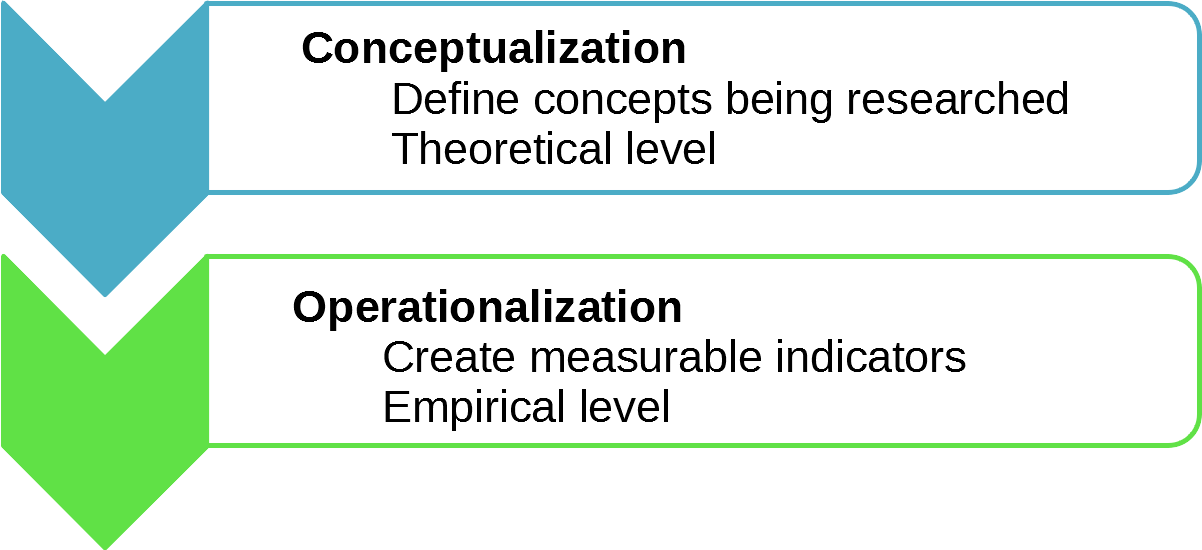
\includegraphics[width=\maxwidth{.95\linewidth}]{gfx/05-ConceptVsOper}
	\caption{Conceptualization Vs. Operationalization}
	\label{05:fig02}
\end{figure}

Indicators operate at the empirical level in contrast to constructs, which are conceptualized at the theoretical level. The combination of indicators at the empirical level representing a given construct are called \glspl{variable}, and up to six types are found in research projects:

\begin{itemize}
	\item Independent variables are those that cause an observed outcome. For example, if a researcher's concept is that older people have more traffic accidents then the independent variable is age.
	\item Dependent variables are those that depend on the independent variable; these are the outcomes of some influence. In the case of the traffic accident concept from above, the dependent variable is the number of traffic accidents.
	\item Intervening (or mediating) variables stand between the dependent and independent variables and mediate the effects of the independent variable. For example, if the research concept is that poor people have shorter lifespans then there must be some sort of intervening variable since poverty, by itself, cannot determine lifespan. In this case, perhaps the intervening variable is lack of access to health care or poorer nutrition.
	\item Moderating variables affect the direction and strength of the relationship between the independent and dependent variables. In medical experiments, for example, the dosage level moderates the outcome (dependent variable) of the medicine (independent variable). 
	\item Control variables are only found in experiments. A control is a subject that has not been exposed to a treatment and is used to compare the outcomes of the treatment. For example, if an experiment is conducted to see if tutoring improves test scores then there must be a control group that does not get tutoring.
	\item Confounding variables are ``extra'' unaccounted variables. If an experiment does not yield the anticipated results researchers will often start searching for a confounding variable that may have influenced the experiment in unexpected ways.
\end{itemize}

Each indicator may have several attributes (or levels) and each attribute represent a value. For instance, a ``gender'' variable may have two attributes: male or female. Likewise, a customer satisfaction scale may be constructed to represent five attributes: ``strongly dissatisfied,'' ``somewhat dissatisfied,'' ``neutral,'' ``somewhat satisfied'' and ``strongly satisfied.'' 

Variables may be quantitative (numeric) or qualitative (textual). Quantitative data can be analyzed using techniques like regression or equation modeling while qualitative data is analyzed with techniques like coding. Note that many variables in business research are qualitative, even when represented with numbers. For instance, imagine a customer satisfaction indicator with five attributes: strongly dissatisfied, somewhat dissatisfied, neutral, somewhat satisfied, and strongly satisfied. If the researcher assigns the numbers $ 1-5 $ respectively for these five attributes then sophisticated statistical tools for quantitative data analysis can be used. However, note that the numbers are only labels associated with respondents' evaluation and the underlying variable (satisfaction) is qualitative.

Indicators may be reflective or formative. A reflective indicator is a measure that ``reflects'' an underlying construct. For example, if religiosity is defined as a construct that measures how religious a person is, then attending religious services may be a reflective indicator of religiosity. A formative indicator is a measure that ``forms'' or contributes to an underlying construct. Such indicators may represent different dimensions of the construct of interest. For instance, if religiosity is defined as composed of a belief dimension, a devotional dimension, and a ritual dimension, then indicators chosen to measure each of these different dimensions will be considered formative indicators. Unidimensional constructs are measured using reflective indicators (even though multiple reflective indicators may be used for measuring abstract constructs such as self-esteem), while multidimensional constructs are measured as a formative combination of the multiple dimensions, even though each of the underlying dimensions may be measured using one or more reflective indicators.

It is important to keep in mind that the process of coming up with indicators cannot be arbitrary or casual. One way to avoid taking an overly casual approach in identifying indicators is to turn to prior theoretical and empirical work. Theories will point to relevant concepts and possible indicators while empirical work will detail specific examples of how key concepts have been measured in the past. One final important detail to think about when deciding on indicators is the strategy you will use for data collection. A survey implies one way of measuring concepts while field research implies a very different way. The data-collection strategy employed will play a major role in shaping how concepts are operationalized.

\section{Measurement Quality}

The previous section examined some of the difficulties with measuring constructs. What makes the task more challenging is that sometimes these constructs are imaginary concepts (\ie, they do not exist in reality), and multi-dimensional (in which case, there is the additional problem of identifying their constituent dimensions). Hence, it is not adequate just to measure constructs using any scale, the scales must be tested to ensure that: 

\begin{enumerate}
	\item they measure the construct consistently and precisely (\ie, the scales are ``reliable'') and 

	\item they actually measure the construct being investigated (\ie, the scales are ``valid''). 
\end{enumerate}

Reliability, the consistency of a measure, and validity, the efficacy of a measure, are the two yardsticks against which the accuracy of measurements are evaluated in scientific research. A measure can be reliable but not valid if it is measuring consistently but it is the wrong construct. Likewise, a measure can be valid but not reliable if it is measuring the right construct but not doing so in a consistent manner. Using the analogy of a shooting target, as shown in Figure \ref{05:fig03}, a measure that is both reliable and valid is like a group that is tightly clustered near the center of the target. A measure that is reliable but not valid is like a group that is tightly clustered but off-center. A measure that is valid but not reliable is a group that is widely scattered but centered. Finally, a measure that is neither reliable nor valid is like a group that is widely scattered and off-center. 

\begin{figure}[H]
	\centering
	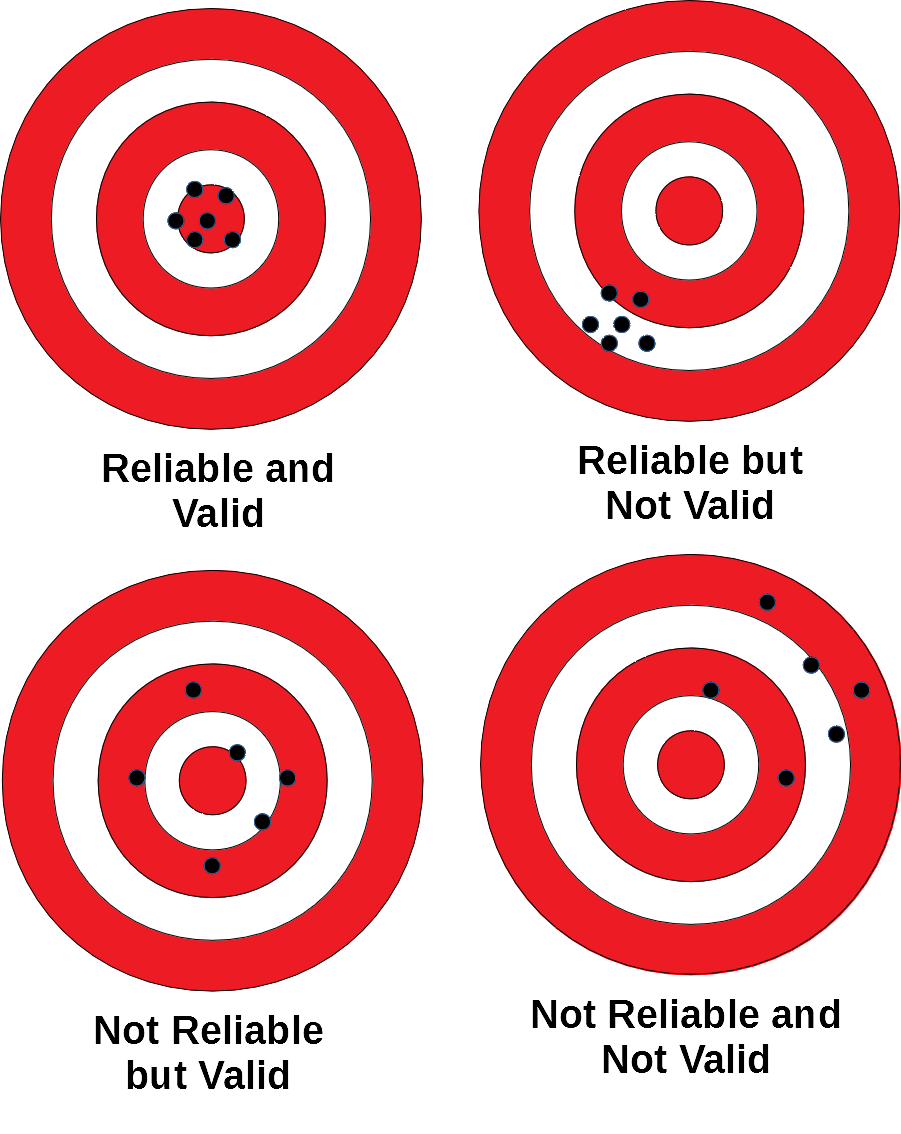
\includegraphics[width=\maxwidth{.95\linewidth}]{gfx/05-Targets}
	\caption{Reliability Analogy}
	\label{05:fig03}
\end{figure}

\subsection{Reliability}

\Gls{reliability} ``...is the extent to which measurements are repeatable – when different persons perform the measurements, on different occasions, under different conditions, with supposedly alternative instruments which measure the same thing.''\cite{drost2011validity}

Any score obtained by a measuring instrument (the observed score) is composed of both the ``true'' score, which is the score that a person would have received if the measurement were perfectly accurate, and the ``error'' in the measurement process. Imagine a simple example, a bathroom scale. If a person's true weight were $ 150 $ pounds then, ideally, the scale would read $ 150 $ every time that person stepped on the scale. The scale's reliability is the consistency of its output from one day to the next. If a person stepped on the scale one day and it read $ 160 $ but the next day it read $ 140 $ then the scale would not be a reliable instrument.

There are two types of reliability errors that researchers need to understand. First is systematic error, one that is caused by the system and is predictable. For example, if the bathroom scale mentioned above constantly read five pounds heavy that would be an error, but it would be one that is consistent and could be corrected in the research analysis. That is an example of a systematic error. The second type of error is a random error. If the bathroom scale were accurate but the person reading it one day read $ 151 $ and the next as $ 145 $ then that would be a random error. Random errors cannot be corrected but tend to cancel out due to the random nature of the error (sometimes the reading will be a bit high and other times low), especially if there are many data points.

Unreliable measurements in business research could be for several reasons. One is the researcher's subjectivity. For example, if employee morale in a firm is being measured by watching whether the employees smile at each other, whether they make jokes, and so forth, then different observers may infer different measures of morale if they are watching the employees on a very busy day (when they have no time to joke or chat) or a light day (when they are more jovial or chatty). Two observers may also infer different levels of morale on the same day, depending on what they view as a joke and what is not. 

``Observation'' is a qualitative measurement technique, but reliability may be improved by using quantitative measures. Counting the number of grievances filed over one month may be a measure of (the inverse of) morale. Of course, grievances may or may not be a valid measure of morale, but it is less dependent on human subjectivity and therefore more reliable. 

A second source of unreliable observation is asking imprecise or ambiguous questions. For instance, if people are asked to report their salary some may state a monthly salary, some an annual salary, and some even an hourly wage. Thus, the resulting observations will be divergent and unreliable. 

A third source of unreliability is asking questions about issues that respondents neither understand nor care about, such as asking an American college graduate about Canada's relationship with Slovenia.

To improve reliability, researchers can replace subjective data collection techniques (observation) with those that are more objective (questionnaire), ask respondents only questions that they may know or care about, avoid ambiguous items (\eg clearly indicate annual salary), and simplify the wording in indicators. While these strategies can improve the reliability of measurements, instruments must still be tested for reliability using techniques like the following.

\begin{itemize}
	\item \textbf{Inter-rater reliability}. Inter-rater reliability, also called inter-observer reliability, is a measure of consistency between two or more independent raters (observers) of the same construct. Usually, this is assessed in a pilot study and can be done in two ways, depending on the level of measurement being used. If the measure is categorical, a set of all categories is defined, raters check off which category each observation falls in, and the percentage of agreement between the raters is used as an estimate of inter-rater reliability. For instance, if there are two raters rating $ 100 $ observations into one of three possible categories, and their ratings match for $ 75\% $ of the observations, then inter-rater reliability is $ 0.75 $. If the measure is interval or ratio scaled (e.g., classroom activity is being measured once every five minutes by two raters on one to seven scale), then a simple correlation between measures from the two raters can also serve as an estimate of inter-rater reliability.

	\item \textbf{Test-retest reliability}. Test-retest reliability is a measure of consistency between two measurements (tests) of the same construct administered to the same sample at two different points in time. If the observations have not changed substantially between the two tests, then the measure is reliable. The correlation in observations between the two tests is an estimate of test-retest reliability. Note here that the time interval between the two tests is critical. Generally, the longer the time gap the greater the chance that the two observations may change during due to random error and the lower the test-retest reliability.

	\item \textbf{Split-half reliability}. Split-half reliability is a measure of consistency between two halves of a construct measure. For instance, if a ten-item test of a given construct is to be administered to a group of subjects then the ten items are randomly split into two sets of five but all ten items are kept in the test. That test is next administered to a sample of respondents. Finally, the score for each group of five questions is calculated for each respondent and the correlation between the two half scores is the split-half reliability. The longer the instrument, the more likely it is that the two halves of the measure will be similar (since random errors are minimized as more items are added), and hence, this technique tends to systematically overestimate the reliability of longer instruments.

	\item \textbf{Internal consistency reliability}. Internal consistency reliability is a measure of consistency between different items of the same construct. If a multiple-item construct measure is administered to respondents, the extent to which respondents rate those items in a similar manner is a reflection of internal consistency. This reliability can be estimated in terms of average inter-item correlation, average item-to-total correlation, or more commonly, \textit{Cronbach’s alpha}. 

\end{itemize}

\subsection{Validity}

\Gls{validity} is concerned with the meaningfulness of research results. In brief, does the research actually measure what it was purported to measure? For example, does the Scholastic Aptitude Test (SAT) actually predict the likelihood of a high school student successfully completing college?\cite{drost2011validity} There are numerous types of validity found in the literature, but they generally form two large groups: Measurement Validity (the measurement should accurately reflect the construct) and Hypothesis Validity (the hypotheses should accurately reflect the construct).

\subsubsection{Measurement Validity}

The \textit{theoretical} assessment of validity focuses on how well an abstract construct is translated into an operational measure, which is called \gls{translationalvalidity}, and divided into two sub-types: face and content validity. Translational validity is typically assessed using a panel of expert judges who rate each item (indicator) on how well it fits the conceptual definition of that construct along with a qualitative technique called \textit{Q-method}, as explained by Pnina Shinebourne\cite{shinebourne2009using}.

The \textit{empirical} assessment of validity examines how well a given measure relates to one or more external criterion, based on empirical observations. This type of validity is called \gls{criterionvalidity}, which is divided into four sub-types: convergent, discriminant, concurrent, and predictive. While translation validity examines whether a measure is a good reflection of its underlying construct, criterion-related validity examines whether a given measure behaves the way it should, given the theory of that construct. The distinction between theoretical and empirical assessment of validity is illustrated in Figure \ref{05:fig04}. However, both approaches are needed to adequately ensure the validity of measures in business research.

\begin{figure}[H]
	\centering
	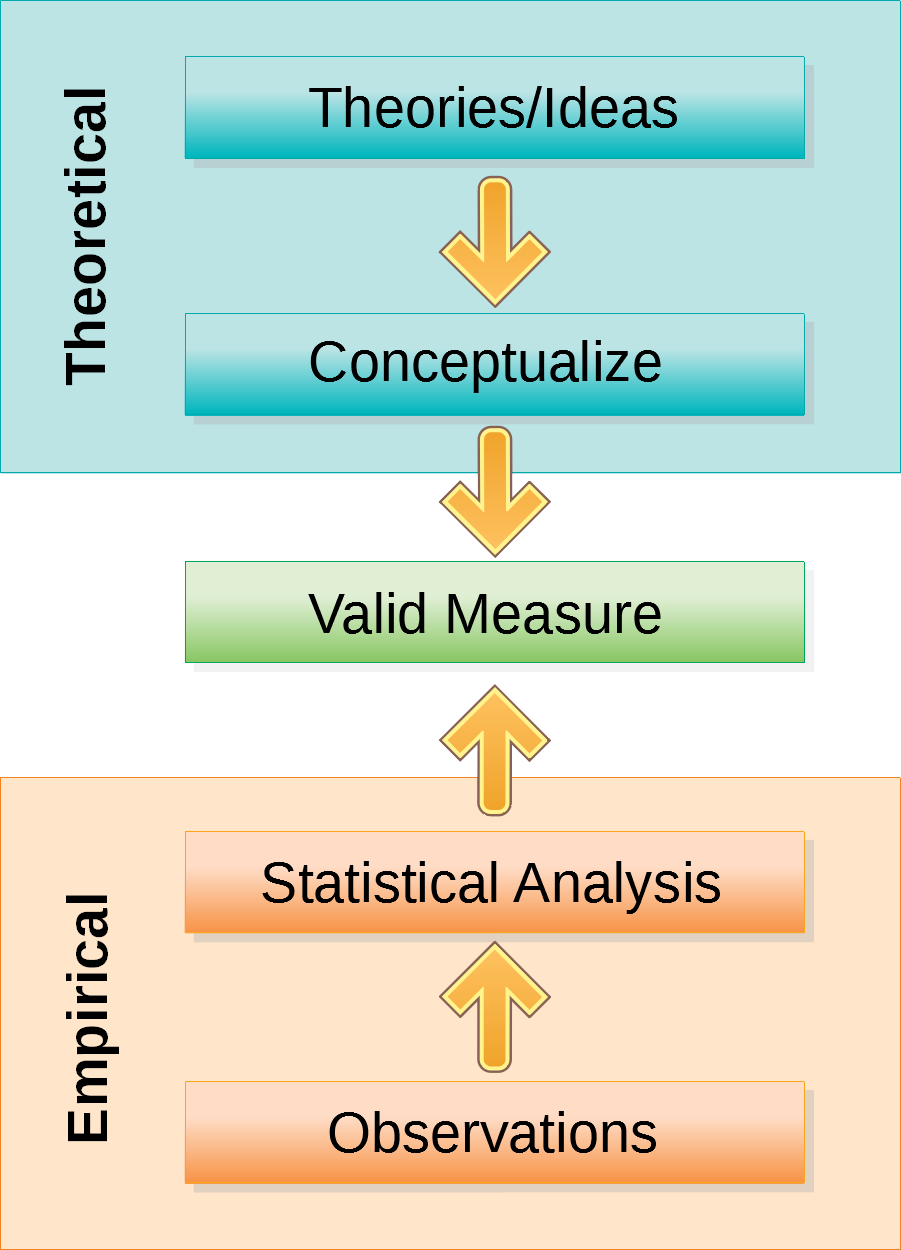
\includegraphics[width=\maxwidth{.95\linewidth}]{gfx/05-AssessValidity}
	\caption{Assessing Theoretical and Empirical Validity}
	\label{05:fig04}
\end{figure}

\paragraph{Translational Validity}

\begin{description}
	\item[\Gls{facevalidity}] refers to whether an indicator seems to be a reasonable measure of its underlying construct ``on its face.'' For instance, the frequency of attendance at religious services seems to make sense as an indication of a person's religiosity without a lot of explanation. Hence this indicator has face validity. However, if it were suggested that the number of books checked out of an office library is a measure of employee morale then such a measure would probably lack face validity because it does not seem to make much sense. Interestingly, some of the popular measures used in organizational research appear to lack face validity, though may have other types of validity. For instance, absorptive capacity of an organization (how much new knowledge can it assimilate for improving organizational processes) has often been measured by research and development intensity (\ie, R\&D expenses divided by gross revenues). Research that includes constructs that are highly abstract or are hard to conceptually separate from each other (\eg, compassion and empathy), may benefit from a panel of experts who can evaluate the face validity of the measures.

	\item[\Gls{contentvalidity}] is an assessment of how well a measure matches the content domain of the construct being measured. For instance, to measure the construct ``satisfaction with restaurant service,'' then the content domain chould include variable like the quality of food, courtesy of wait staff, duration of wait, and the overall ambiance of the restaurant (i.e., whether it is noisy, smoky, etc.). Of course, this approach assumes the researcher can create a detailed description of the content domain, which may be difficult for complex constructs such as self-esteem or intelligence. As with face validity, an expert panel of judges may be employed to examine content validity of constructs.
\end{description}

\paragraph{Criterion-Related Validity}

\begin{description}

	\item[\Gls{convergentvalidity}] refers to the closeness with which a measure, or group of measures, relates to (or converges on) the construct that it is purported to measure. Convergent validity can be established by comparing the observed values of one indicator with those of other indicators to attempt to find high correlation between those indicators. Compare this to discriminant validity.
	
	\item[\gls{discriminantvalidity}] refers to the degree to which a measure does not measure (or discriminates from) other constructs that it is not supposed to measure. Usually, convergent validity and discriminant validity are assessed jointly for a set of related constructs. For example, if an organization's knowledge is related to its performance then a measure of organizational knowledge must actually measure organizational knowledge (convergent validity) and not organizational performance (discriminant validity). Discriminant validity is established by demonstrating that indicators of one construct are dissimilar from (\ie, have low correlation with) other constructs.

	\item[\Gls{concurrentvalidity}] examines how well a measure of one outcome relates to another outcome that is presumed to occur simultaneously. For instance, do students' scores in a calculus class correlate well with their scores in a linear algebra class? Since both are mathematics classes it would be presumed that there is high concurrent validity between scores in those classes. 
	
	\item[\Gls{predictivevalidity}] is the degree to which a measure successfully predicts a future outcome. For example, a standardized test score (\eg, \textit{Scholastic Aptitude Test}) can be used to predict a student's academic success in college. Concurrent and predictive validity are not often considered in empirical business research.

\end{description}

\subsubsection{Hypothesis Validity}

In general, four types of hypothesis validity are referred to in the literature.

\begin{description}
	\item[\Gls{internalvalidity}] examines whether the observed change in a dependent variable is caused by a corresponding change in hypothesized independent variable and not by variables extraneous to the research context. This is sometimes called ``causality'' and it requires three conditions: 
	
	
	\begin{enumerate}
		\item covariation of cause and effect (if cause happens then effect also happens and if cause does not happen effect does not happen)
		\item temporal precedence (cause must precede effect in time)
		\item lack of plausible alternative explanation (or spurious correlation). 
	\end{enumerate}
	
	Certain research designs, such as laboratory experiments, are strong in internal validity since researchers can manipulate the independent variable (cause) via a treatment and observe the effect (dependent variable) of that treatment after a certain point in time while controlling for the effects of extraneous variables. Other designs, such as field surveys, are poor in internal validity because researchers cannot manipulate the independent variable (cause) and because cause and effect are measured at the same point in time which defeats temporal precedence making it equally likely that the effect actually brought about the presumed cause rather than the reverse. 
	
	\item[\Gls{externalvalidity}] \marginpar{Some researchers claim that increased external validity leads to decreased internal validity and vice-versa, but this is not always true. Some research designs, such as multiple case studies, have high degrees of both internal and external validities.}refers to whether the observed associations can be generalized from the sample to the population (population validity), or to entities outside the population (ecological validity). For example, if results drawn from a sample of financial firms in the United States can be generalized to the population of all financial firms it would have strong population validity and if to other types of firms it would have strong ecological validity. Survey research, where data are sourced from a wide variety of individuals, firms, or other units of analysis, tends to have broader generalizability than laboratory experiments where artificially contrived treatments and strong control over extraneous variables render the findings less generalizable to real-life settings where treatments and extraneous variables cannot be controlled. 
	
	\item[\Gls{constructvalidity}] examines how well a given measurement scale is measuring the theoretical construct that it is designed to measure. One frequent problem with construct validity is simply defining the construct in such a way that it is measurable. As one example, ``property ownership'' is a construct of a market economy explained by Robert Reich\cite{reich2016saving}. That is, the fact that people can own property drives a local economy. But this construct relies on a number of external forces that cannot be controlled, such as local politics (a city's eminent domain can take a person's property) and the value of the property on the open market. Measuring the influence of property ownership on a local economy (the construct) would be very difficult since there are so many confounding variables. 
	
	\item[\Gls{statisticalvalidity}] examines the extent to which conclusions derived from a statistical procedure are valid. For example, it examines whether the right statistical method was used and whether the variables meet the assumptions of that statistical test (such as sample size or distributional requirements). 
	
\end{description}

\subsection{Improving Internal and External Validity}

The best research designs are those that can assure high levels of internal and external validity. Such designs would guard against spurious correlations, inspire greater faith in the hypotheses testing, and ensure that the results drawn from a small sample are generalizable to the population at large. The internal validity of research designs and can be improved using four methods.

\begin{enumerate}
	\item \textbf{Manipulation} involves the researcher manipulating the independent variables in one or more ways (called ``treatments''), and compares the effects of the treatments against a control group where subjects do not receive the treatment. Treatments may include a new drug or different dosage of drug (for treating a medical condition), a new teaching style (for education), and so forth. This type of control can be achieved in experimental or quasi-experimental designs but not in non-experimental designs such as surveys. 
	
	\item \textbf{Elimination} relies on eliminating extraneous variables by holding them constant across treatments, such as by restricting the study to a single gender or a single socioeconomic status. 
	
	\item \textbf{Inclusion} is the process of separately estimating the effects of spurious variables on the dependent variable. As an example, consider the process of estimating the effect of gender on a marketing study. Inclusion techniques allow for greater generalizability of the study but also require substantially larger samples. 
	
	\item \textbf{Randomization} is aimed at canceling out the effects of extraneous variables through a process of random sampling. Two types of randomization are: 1) random selection, where a sample is selected randomly from a population, and 2) random assignment, where subjects selected in a non-random manner are randomly assigned to treatment groups. Randomization also improves external validity, allowing inferences drawn from the sample to be generalized to the population from which the sample is drawn; however, generalizability across populations is harder to ascertain since populations may differ on multiple dimensions and only a few of those dimensions can be controlled.
	
\end{enumerate}

\begin{figure}[H]
	\centering
	
\includegraphics[width=\maxwidth{.95\linewidth}]{gfx/Sampling_Of_Research}
	\caption*{}
	\label{05:sampling_of_research}
\end{figure}
\section{A Sampling of Research}

\subsection{Consumer Self-Confidence}

Bearden, Hardesty, and Rose investigated consumer self-confidence in $ 2001 $\cite{bearden2001consumer}. The goal of their research project was to refine the conceptualization and measurement of consumer self-confidence in order to provide a better understanding of that concept. Consumer self-confidence is defined as, ``\ldots the extent to which an individual feels capable and assured with respect to his or her marketplace decisions and behaviors.'' The researchers conceptualized consumer self-confidence as two higher-order factors that are each made up of several dimensions.

\begin{itemize}
	\item Decision-Making Self-Confidence
	\begin{itemize}
		\item Information acquistion and processing. Assessed with statements like, ``I know where to find the information I need prior to making a purchase'' and ``I know the right questions to ask when shopping.''
		\item Consideration-Set formation. Assessed with statements like, ``I can tell which brands meet my expectations'' and ``I know which stores to shop.''
		\item Personal outcomes. Assessed with statements like, ``I frequently agonize over what to buy'' and ``I never seem to buy the right thing for me.''
		\item Social outcomes. Assessed with statements like, ``I have the ability to give good presents'' and ``I impress other people with the purchases I make.''
	\end{itemize}
	\item Protection
	\begin{itemize}
		\item Persuasion Knowledge. Assessed with statements like, ``I know when an offer is 'too good to be true''' and ``I can separate fact from fantasy in advertising.''
		\item Marketplace Interfaces. Assessed with statements like, ``I am hesitant to complain when shopping'' and ``I have a hard time saying no to a salesperson.''
	\end{itemize}
\end{itemize}

After the conceptualization and measurement phase, the researchers completed seven different studies designed to affirm the reliability and validity of their work. The first step was to create a pool of $ 145 $ items generated from exploratory interviews with $ 43 $ adult consumers. The items were screened to reduce redundancy and the remaining items were given to an expert panel of $ 14 $ marketing faculty members in a major university. That reduced the pool of statements to $ 97 $.

The pool of $ 97 $ statements were used in the form of a survey for two different studies, one to $ 221 $ and the other to $ 204 $ adults. After that data were gathered, factor analysis was used to eliminate items that were determined to not contribute significantly to the concept or were unclear. This reduced the pool to $ 39 $ items. 

A third study was completed where the $ 39 $ items were administered to $ 252 $ undergraduate business students. The results of that study indicated that a two-factor higher-order model with six-factor dimensions (as noted above) best fit the data. At this point, the researchers determined that the reliability and discriminant validity were both high.

For study four and five the researchers tested their model for test-retest reliability, convergent validity, and relative predictive validity. They found the model performed well on each of these criteria. Study six was designed to test the model to see if it would detect known group differences, and it did.

One final study was conducted where the model was tested with $ 106 $ faculty and staff members from a large state university. They were asked to decide which of several competing products they would purchase based on price and perceived quality. The researchers found that consumers who had higher self-confidence tended to select the more expensive product but chose to defer the purchase when the self-confidence level was lower.

This study is an excellent example of how researchers generate a concept and determine how to measure that concept. That measurement is then subjected to extensive testing to ensure its reliability and validity.



\subsection{Validity in Qualitative Research Revisited}

The validity measures in this chapter have been designed, primarily, for quantitative research. For many years researchers have had concerns with the validity of qualitative studies. To answer those concerns, qualitative research project often assure ``validity'' by using some tortured form of validity used in quantitative project (as described earlier in this chapter). Cho and Trent revisited the concept of validity in qualitative research and propose a recursive, process-oriented view of validity\cite{cho2006validity}.

The researchers first define the two current qualitative validity.

\begin{itemize}
	\item Transactional. This is an interactive process between the researcher, the researched, and the collected data that is aimed at achieving a relatively higher level of accuracy and consensus. This approach assumes that qualitative research can be more credible as long as certain techniques, methods, and/or strategies are employed during the conduct of the inquiry. The major ways this validity is performed is with ``member checking'' (reassuring the credibility of the participants) and triangulation (verifying facts using multiple data sources).
	\item Transformational. This is a progressive process leading toward social change that is to be achieved by the research endeavor itself. It acknowledges that qualitative researchers emphasize the value-laden nature of social interactions and multiple perspectives on a topic would yield multiple meanings. Qualitative researchers would assert that a positivest inquiry is not that absolute truth but merely one facet of the truth. The validity of this type of study is found through self-reflection where the researchers deconstruct/reconstruct the meanings attached to their findings in order to make them more fruitful. 
\end{itemize}

Cho and Trent then argue that the two traditional approaches are not adequate measures of validity for qualitative research projects and propose, instead, to extend Donmoyer's framework of ``five overarching purposes undergirding contemporary qualitative research.''\cite{donmoyer2001paradigm} 

\begin{itemize}
	\item Validity in the ``truth'' seeking purpose. Finding ``truth'' is, perhaps, the ultimate goal for any research project, but Cho and Trent maintain that there is not a single measure that will validate the truthfulness of some finding. Instead, they propose that ``'truth' seeking purpose is progressive induction through which data need to be collected, analyzed, interpreted, triangulated, and thus represent 'what is' through a credible, corresponding 	account.'' They believe that member checking and triangulation, as described above, fill this purpose.
	\item Validity in the thick description purpose. Qualitative research often does not intend to find ``truth'' as in a quantitative project; instead, the goal is to explain the unique perspectives constructed by individuals and groups. Thus, the outcome for many qualitative research projects is a ``thick description'' of some phenomenon in the form of a case study or ethnography. Validity in this purpose is achieved through holistic and prolonged engagement between the researcher and the subject being studied. The validity is a result of the extent to which data are presented (``let readers see for themselves'') and the researcher's competence in interpreting what was found.
	\item Validity in the developmental purpose. Often, a qualitative research project concerns observing the shared interests of individuals or groups as those interests develop over time. These types of projects may be little more than a comprehensive investigation of what happens over time or as involved as explaining how things make progress stage by stage. Validity is assured by transactional means (as described above), but ongoing as the project unfolds rather than a single process completed at the end of the project.
	\item Validity in the personal essay purpose. This type of qualitative research project is similar to a thick description, but is intentionally and openly subjective. The researcher tells a personal story and reflects on lessons learned in that process. Validity is gained through the expertise of the researcher in the field being explored. This type of research is sometimes called ``autoethnography.'' For example, a research project where professional actors reflect on the art of acting would have a high degree of validity.
	\item Validity in the praxis/social change purpose. Some qualitative research projects include as a goal the desire to bring about change. This is especially true in ``action research'' projects, as covered in Chapter \ref{ch13:interpretive_research}. This type of research is more frequently found in educational than business settings. Validity is assured through three methods: member checks, researchers thinking critically about their own involvement in the project, and whether the status quo was redefined.
\end{itemize}

Cho and Trent close their work by describing the holistic requirement of validating a study. They believe that it is not adequate to simply provide member checks and triangulation, rather, ``\ldots we are proposing an inclusive discourse of validity in qualitative research by reflecting on what matters specific to the problem/research within our research purview.'' They believe that a narrative which explains the approaches to validity taken by the researchers is best so readers can judge for themselves if the research is valid. Their conclusion includes this statement:

\begin{quote}
	Many are interested in creating new senses of validity in qualitative research. Some hope that validity methods and strategies in qualitative research can be defined to the extent that they are equal to those of conventional or quantitative research methods. We believe this to be a misguided aim. We add that a variety of purposeful approaches (e.g. thick description and praxis/social change) may be combined to obtain holistically 'valid' results.
\end{quote}

Figure \ref{05:fig05} is based on one presented by Cho and Trent in this report.

\begin{figure}[H]
	\centering
	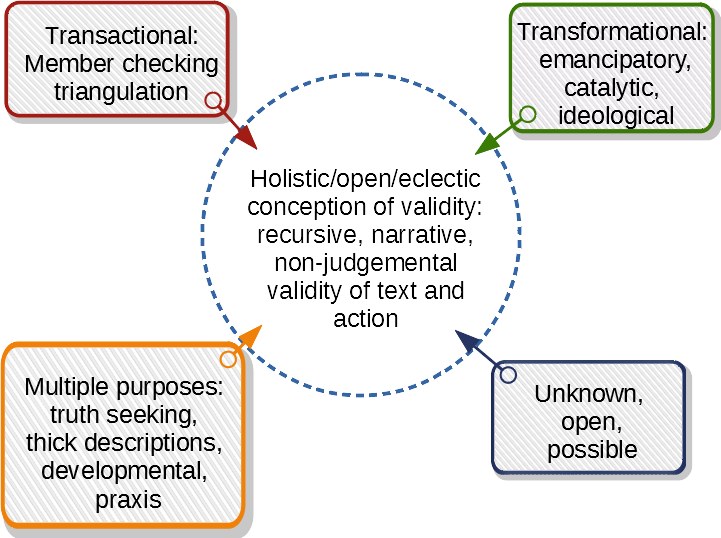
\includegraphics[width=\maxwidth{.95\linewidth}]{gfx/05-cho}
	\caption{Validity for Qualitative Research}
	\label{05:fig05}
\end{figure}

\section{Summary}\label{ch05:summary}

\begin{center}
	\begin{tkawybox}{Summary}
		\begin{itemize}
			\setlength{\itemsep}{0pt}
			\setlength{\parskip}{0pt}
			\setlength{\parsep}{0pt}
			
			\item Defining measurement
			\item Distinguishing between conceptualization and operationalization
			\item Defining reliability and validity 
			\item Compare and contrast reliability and validity
			\item Improving both reliability and validity in research projects
		\end{itemize}
	\end{tkawybox}
\end{center}
